\chapter{Gomolakowie z~Wnętrznego i~Gomołowie z~Mysłowa}

% Przednia okładka podrozdziału
\includepdf{Wnętrzne_mapa_fin.png}

\section{Wnętrzne: 1714~r. - 1783~r.}

Wieś Wnętrzne w~XVIII~wieku znajdowała się na granicy województw lubelskiego, 
mazowieckiego i~sandomierskiego, zaliczana była do ziemi łukowskiej. 
Najbliższymi dużymi ośrodkami miejskimi dla Wnętrznego były: oddalony 
o~około 25~kilometrów na wschód Łuków oraz oddalony o~około 35~kilometrów na 
zachód Garwolin. Wieś ta należała w~tamtym czasie do parafii 
rzymskokatolickiej pod wezwaniem Niepokalanego Serca Najświętszej Maryi Panny 
w~Wilczyskach. Wnętrzne zostało założone prawdopodobnie pomiędzy 1531 
a~1552~rokiem - wynika to zapisów rejestrów poborowych województwa 
lubelskiego \cite{apawinski}. W~rejestrze z~1531~roku do nowo założonej 
parafii Wilczyska (parafia erygowana w~1505~roku) przypisane są tylko 
trzy~wsie: Mysłów, Lisikierz oraz Wola Mysłowska, natomiast rejestr 
z~1552~roku wskazuje już siedem wsi przynależących do parafii w~Wilczyskach, 
były nimi: Mysłów, Lisikierz, Wola Mysłowska, Wnętrzne, Kamień, Osiny Nowe 
oraz Grudź Nowa (patrz: ryc. \ref{fig:wilczyska_1552}). W~XVI~wieku 
właścicielami wyżej wymienionych wsi były rodziny Mysłowskich i~Morawców, 
jednak pod koniec XVIII~wieku wsie te stanowiły już część pokaźnego majątku 
rodziny Rzewuskich (herbu Krzywda), a~konkretnie ich właścicielem był Tomasz 
Rzewuski, chorąży łukowski. 
\nocite{sulimierski}

\begin{figure}[!ht]
    \vspace*{0.5cm}
    \centering 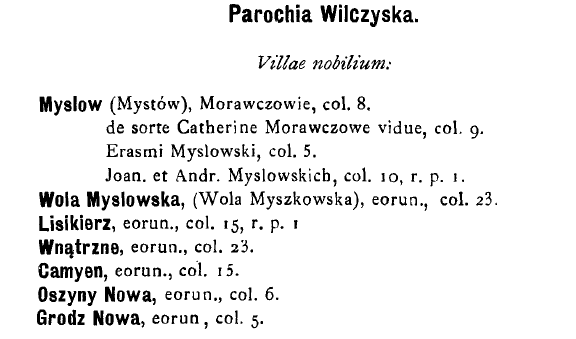
\includegraphics[width=0.7\linewidth]{Wilczyska_1552.png}
    \captionsetup{format=hang}
    \caption{Wpis dotyczący parafii Wilczyska pochodzący z~rejestrów 
    poborowych województwa lubelskiego z~1552~roku \cite{apawinski}.}
    \label{fig:wilczyska_1552}
\end{figure}

Księgi metrykalne parafii Wilczyska pochodzące z~XVIII wieku, nie były, 
w~momencie pisania niniejszej książki, dostępne w~formie cyfrowej, nie 
możliwe było również uzyskanie do nich dostępu kontaktując się bezpośrednio 
z~parafią, gdyż parafia Wilczyska, podobnie jak parafia Zbuczyn, należy do 
diecezji siedleckiej, która nie zezwala na udostępnianie osobom prywatnym tak 
wiekowych akt. Jedynym dostępnym, w~momencie pisania niniejszej książki, 
źródłem wiedzy o~chrztach, ślubach oraz zgonach w~parafii Wilczyska 
w~XVIII~wieku były wpisy w~bazie indeksów metrykalnych Lubelszczyzny - 
\emph{Lubgens}, sporządzone przez grupę indeksacyjną \emph{Lubelskie 
Korzenie}\footnote{
    \url{https://regestry.lubgens.eu/viewpage.php?page_id=1052&par=112} 
    (dostęp: marzec 2024 r.).}. Baza Lubgens zawierała, w~momencie pisania 
    niniejszej książki, informacje o~osobach ochrzczonych w~parafii Wilczyska 
    w~latach 1620-1919, o~osobach, które zawarły związek małżeński w~tej 
    parafii w~latach 1620-1919 oraz o~osobach zmarłych w~latach 1740-1919. 
    W~formie cyfrowej, na portalu \emph{szukajwarchiwach.gov.pl}, dostępne 
    są natomiast księgi metrykalne parafii Wilczyska z~lat 
    1810-1921\footnote{Akta te dostępne są pod adresami: \\ 
    \url{https://www.szukajwarchiwach.gov.pl/en/zespol/-/zespol/4383} 
    (dostęp: marzec 2024 r.) \\ 
    \url{https://www.szukajwarchiwach.gov.pl/en/zespol/-/zespol/56776} 
    (dostęp: marzec 2024 r.).}.

\begin{figure}[!ht]
    \vspace*{0.5cm}
    \centering 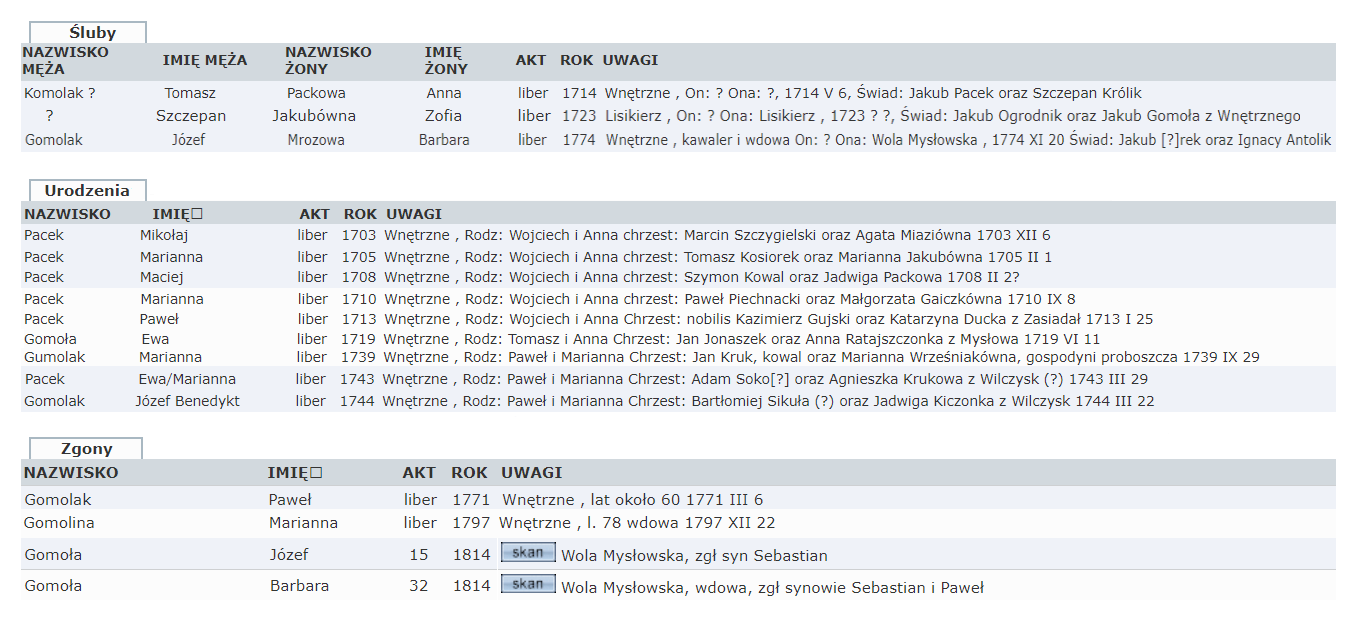
\includegraphics[width=1.0\linewidth]{
        Pacek_Gomołowie_Wnętrzne_wpisy_Lubgens.png}
    \captionsetup{format=hang}
    \caption{Wpisy w~bazie indeksów metrykalnych \emph{Lubgens} dotyczące 
    rodziny Tomasza Gomolaka zamieszkałej we wsi Wnętrzne na początku 
    XVIII~wieku.}
    \label{fig:pacek_gomola_lubgens}
\end{figure}

Pierwszą linią osób posługujących się nazwiskiem Gomolak / Gomoła / Gomuła, 
która pojawiła się we wsi Wnętrzne na początku XVIII~wieku była linia 
zapoczątkowana przez Tomasza Gomolaka (Gomołę). Tomasz Gomolak ożenił się 
w~1714~roku w~Wilczyskach z~Anną Packówną (patrz: ryc. 
\ref{fig:pacek_gomola_lubgens}) - w~bazie \emph{Lubgens} został 
prawdopodobnie mylnie określony jako \enquote{Komolak~?}. Oboje wywodzili się 
ze stanu chłopskiego\footnote{Wpisy w~bazie \emph{Lubgens}, podobnie jak akta 
parafialne parafii Zbuczyn, wyraźnie wskazują na pochodzenie stanowe rodziców 
nowo narodzonych dzieci, nowożeńców biorących ślub, czy osób zmarłych - osoby 
ze stanu szlacheckiego tytułowane są zazwyczaj łacińskim zwrotem 
\emph{nobilis} lub \emph{generosus} w~przypadku bogatszych szlachciców}. Anna 
Pacek była wdową po Wojciechu Packu, z~którym miała piątkę dzieci: Mikołaja 
(ur. 1703~r.), Mariannę (ur. 1705~r.), Macieja (ur. 1708~r.), Mariannę 
(ur. 1710~r.) oraz Pawła (ur. 1713~r.) - nie wiadomo ile dzieci z~pierwszego 
małżeństwa Anny dożyło dorosłości, na pewno jej najmłodszy syn Paweł (urodził 
się rok przed drugim ślubem swojej matki) przyjął nazwisko Gomolak / Gomoła 
po swoim ojczymie i~posługiwał się nim aż do śmierci. Z~małżeństwa Tomasza 
Gomolaka i~Anny Pacek, w~1719~roku, urodziła się Ewa Gomoła (patrz: ryc. 
\ref{fig:pacek_gomola_lubgens}), która była pierwszą osobą o~tym nazwisku, 
która urodziła się we wsi Wnętrzne. Dalsze losy Ewy Gomoły nie są znane, 
wiadomo natomiast, iż Paweł Pacek vel Gomolak, pasierb Tomasza Gomolaka, miał 
trójkę dzieci, które odziedziczyły po nim nazwisko Gomolak / Gomoła: 
Mariannę\footnote{W bazie \emph{Lubgens} została mylnie wpisana jako 
Gumolak.} (ur. 1739~r.), Ewę Mariannę\footnote{W~bazie \emph{Lubgens} zostało 
jej wpisane nazwisko Pacek, czyli pierwsze nazwisko jej ojca.} (ur. 1743~r.) 
oraz Józefa Benedykta (ur. 1744~r.). Józef Benedykt Gomoła jest założycielem 
linii Gomołów, którzy do dnia dzisiejszego żyją w~Woli Mysłowskiej (wieś 
oddalona od Wnętrznego o~około 12~kilometrów na zachód), gdzie przeprowadził 
się w~1774~roku po ślubie z~Barbarą Mróz (z~domu Dudzik) - razem dochowali 
się dziewiątki dzieci.

\begin{figure}[!ht]
    \vspace*{0.5cm}
    \centering 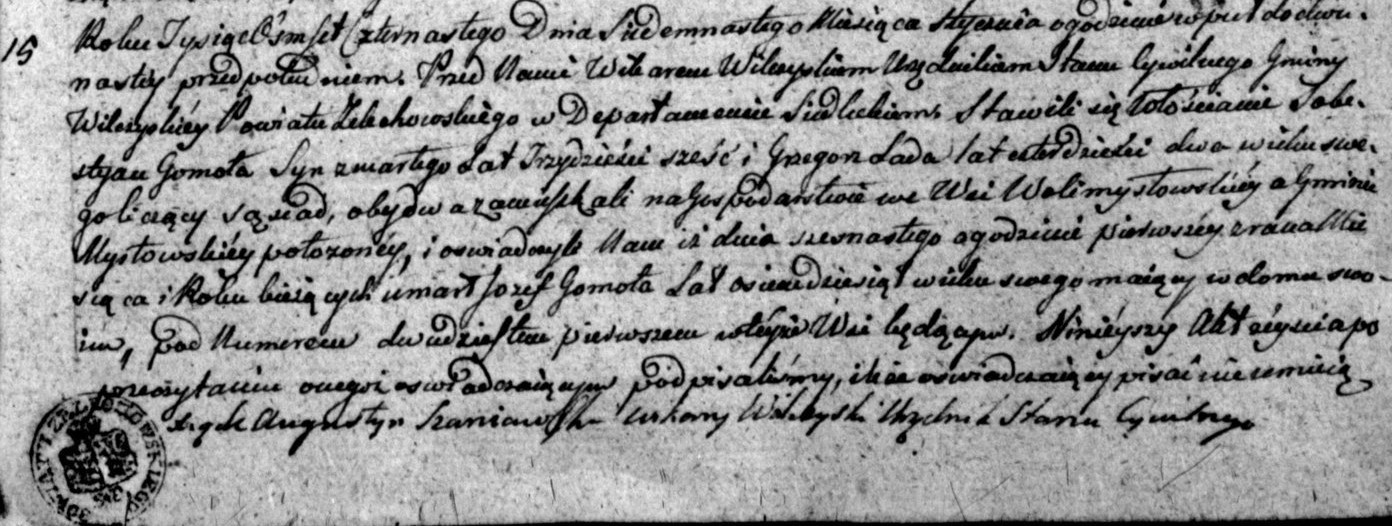
\includegraphics[width=1.0\linewidth]{
        1814_Józef_Benedykt_Gomoła_akt_zgonu_parafia_Wilczyska_wpis_15.jpg}
    \captionsetup{format=hang}
    \caption{Akt zgonu Józefa Benedykta Gomoły - par. Wilczyska 1814~rok 
    (15/1814) \cite{par_wilczyska1}.}
    \label{fig:jbgomola}
\end{figure}

\begin{figure}[!ht]
    \vspace*{0.5cm}
    \centering \includegraphics[width=1.0\linewidth]{
        1814_Barbara_Gomoła_akt_zgonu_parafia_Wilczyska_wpis_32.jpg}
    \captionsetup{format=hang}
    \caption{Akt zgonu Barbary Gomoły - par. Wilczyska 1814~rok (32/1814) 
    \cite{par_wilczyska1}.}
    \label{fig:bgomola}
\end{figure}

Czy można Tomasza Gomolaka vel Gomoła odnaleźć wśród gałęzi rodziny 
Dziewulskich z~Dziewul posługującej się przydomkami Gomolak / Gomolik / 
Gomoła / Gomuła? Niestety, bez dostępu do akt parafii Zbyczyn z~końcówki 
XVII~wieku nie jesteśmy w~stanie stwierdzić czy osoba o~tym imieniu 
i~przydomku urodziła się w~Dziewulach przed 1700~rokiem. Być może był on 
synem Jakuba Dziewulskiego Gomolika - w~akcie jednego ze ślubów w~Wilczyskach 
z~1723 roku jako świadka podaje się Jakuba Gomołę z Wnętrznego (patrz: ryc. 
\ref{fig:pacek_gomola_lubgens}), być może Tomasz przybył do Wnętrznęgo wraz 
ze swoim ojcem Jakubem po tym jak opuścili rodzinną wieś Dziewule tracąc 
tytuł szlachecki i~rodowe nazwisko? Na bazie obecnie dostępnych dokumentów 
nie jesteśmy w~stanie tego rozstrzygnąć. Nie można jednak zignorować faktu, 
iż Tomasz Gomolak vel Gomoła posługiwał się dwoma z~czterech 
charakterystycznych przydomków dla jednej z~gałęzi rodziny Dziewulskich oraz 
faktu, iż po jego przybyciu do Wnętrznego, we wsi tej zaczęli pojawiać się 
kolejni chłopi o~nazwiskach Gomolak / Gomoła / Gomuła, którzy nie urodzi się 
na terenie parafii Wilczyska.

\begin{figure}[!ht]
    \vspace*{0.5cm}
    \centering \includegraphics[width=0.9\linewidth]{
        1812_Jadwiga_Kruk_Gomoła_akt_zgonu_parafia_Wilczyska_wpis_1.jpg}
    \captionsetup{format=hang}
    \caption{Akt zgonu Jadwigi Kruk z~d.~Gomoły - par. Wilczyska 1812~rok 
    (1/1812) \cite{par_wilczyska1}.}
    \label{fig:jgomola_1812}
\end{figure}

\begin{figure}[!ht]
    \vspace*{0.5cm}
    \centering 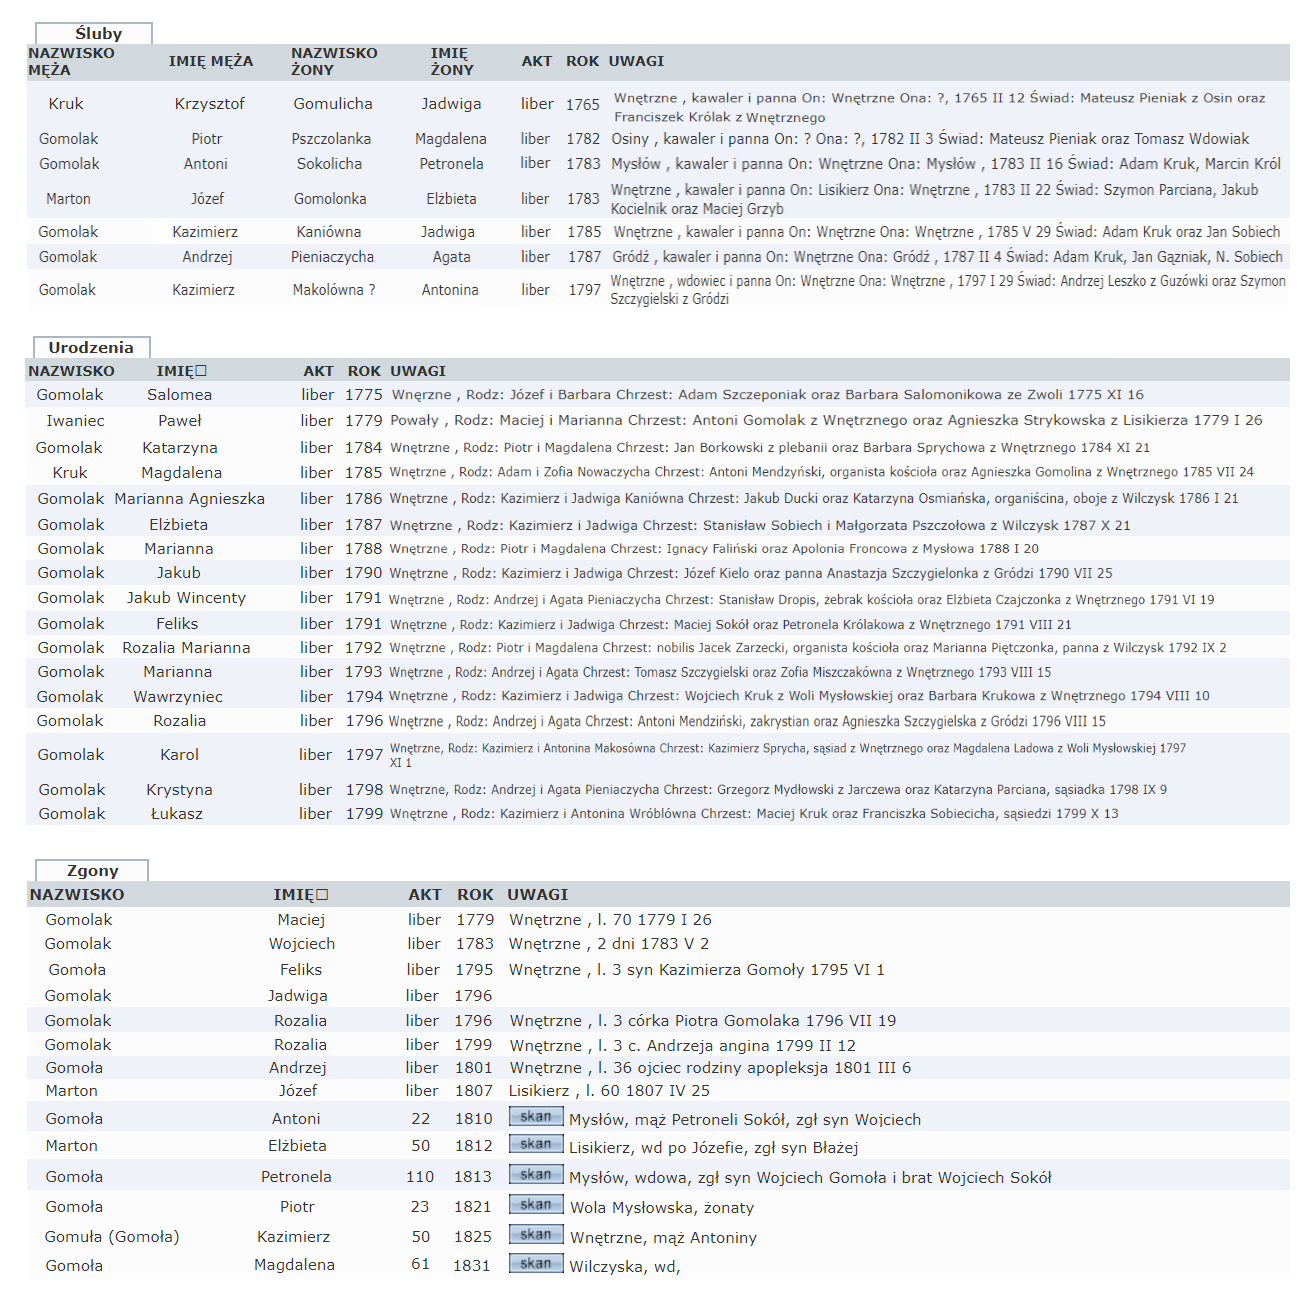
\includegraphics[width=1.0\linewidth]{
        Gomołowie2_Wnętrzne_wpisy_Lubgens.png}
    \captionsetup{format=hang}
    \caption{Wpisy w~bazie indeksów metrykalnych \emph{Lubgens} dotyczące 
    Gomolaków, którzy osiedlili się we wsi Wnętrzne w~końcówce XVIII~wieku.}
    \label{fig:gomola2_lubgens}
\end{figure}

Druga fala osiedleń Gomołów we Wnętrznym rozpoczęła się około 1765~roku,
50~lat od przybycia pierwszych Gomolaków do tej miejscowości. 12~lutego 
1765~roku w~Wilczyskach Jadwiga Gomulicha wzięła ślub z~Krzysztofem Krukiem 
(patrz: ryc. \ref{fig:gomola2_lubgens}) - z~wpisów w~bazie indeksów 
metrykalnych \emph{Lubgens} wynika, iż oboje wywodzili się ze stanu 
chłopskiego. Nie sposób jest odnaleźć aktu narodzin Jadwigi Gomoły w~parafii 
w~Wilczyskach, według aktu jej zgonu dożyła ona wieku około 80~lat, umierając 
w~1812~roku (patrz: ryc. \ref{fig:jgomola_1812}), co oznaczałoby, że urodziła 
się około 1730~roku. W~1728~roku w~Dziewulach narodziła się Jadwiga 
Dziewulska Gomolik, córka Macieja i~Ewy Dziewulskich Gomolików (patrz: ryc. 
\ref{fig:jgomola_1728}), być może przybyła ona do Wnętrznego razem ze swoim 
ojcem Maciejem - według akt zgonów parafii Wilczyska, w~1779~roku we wsi 
Wnętrzne zmarł Maciej Gomolak (patrz: ryc. \ref{fig:gomola2_lubgens}), 
w~wieku około 70~lat (nikt o~takim imieniu i~nazwisku nie urodził się 
w~wilczyńskiej parafii około 1700~roku), co odpowiadałoby mniej 
więcej\footnote{Wiek podawany w~aktach zgonu w~tamtych czasach był zazwyczaj 
wiekiem przybliżonym, szczególnie dla osób ze stanu chłopskiego, zmarłych 
w~podeszłym wieku, gdyż osoby zgłaszające zgon nie znały często dokładnej 
daty urodzenia denata, często sam niepiśmienny denat jej nie znał.} wiekowi 
Macieja Dziewulskiego Gomolika, urodzonego w~1703~roku w~Dziewulach (patrz: 
ryc. \ref{fig:mgomola_1703}). Nie można mieć pewności, iż Jadwiga i~Maciej 
Gomolakowie z~Wnętrznego, należący do stanu chłopskiego, to zubożali drobni 
szlachcice Jadwiga i~Maciej Dziewulscy Gomolikowie z~Dziewul, istnieją jednak 
przesłanki, iż ta zbieżność imion i~dat narodzin może nie być przypadkowa.

\begin{figure}[!ht]
    \vspace*{0.5cm}
    \centering \includegraphics[width=1.0\linewidth]{
        1810_Antoni_Gomoła_akt_zgonu_parafia_Wilczyska_wpis_22.jpg}
    \captionsetup{format=hang}
    \caption{Akt zgonu Antoniego Gomoły - par. Wilczyska 1810~rok (22/1810) 
    \cite{par_wilczyska1}.}
    \label{fig:agomola}
\end{figure}

Kolejną chronologicznie osobą o nazwisku Gomoła / Gomolak / Gomuła, która 
pojawia się we Wnętrznym oraz jest wspomniana w~aktach metrykalnych parafii 
Wilczyska, jest \textbf{Antoni Gomolak}, który w~1779~roku jest wymieniony 
jako ojciec chrzestny Pawła Iwańca - \enquote{...Chrzest: Antoni Gomolak 
z~Wnętrznego...} (patrz: ryc. \ref{fig:gomola2_lubgens}). Antoni jest kolejną 
omawianą w~niniejszym rozdziale osobą, która prawdopodobnie urodziła się poza 
parafią pod wezwaniem Niepokalanego Serca Najświętszej Maryi Panny 
w~Wilczyskach - osoba o~takim imieniu i~nazwisku nie występuje w~tamtejszych 
aktach parafialnych przed 1779~rokiem. Dnia 16~lutego 1783~roku Antoni Gomoła 
ożenił się z~pochodzącą z~pobliskiej wsi Mysłów \textbf{Petronellą Sokół} 
(urodzoną około 1768~roku) - z~wpisów w~bazie indeksów metrykalnych 
\emph{Lubgens} wynika, iż oboje pochodzili ze stanu chłopskiego. Po ślubie 
zamieszkują wspólnie w~rodzinnej miejscowości Petronelli, dochowując się 
dziewiątki dzieci. Z~aktu zgonu Antoniego Gomoły z~1810~roku (patrz: ryc. 
\ref{fig:agomola}) wynika, iż w~momencie śmierci miał on 46~lat, co by 
oznaczało, iż urodził się około 1764~roku. W~związku z~tym, iż akta osób 
ochrzczonych w~parafii Zbuczyn z~lat 1750-1765 nie są dostępne, niemożliwe 
obecnie jest sprawdzenie, czy we wsi Dziewule około 1765~roku urodziła się 
osoba o~imieniu Antoni, nazwisku Dziewulski, nosząca jeden z~przydomków 
Gomoła / Gomolak / Gomuła / Gomolik. \textbf{To co wiemy na pewno to fakt, iż 
Antoni Gomoła i~Petronella Sokół są protoplastami rodziny Gomulskich, nie 
nosili oni wprawdzie nigdy nazwiska \enquote{Gomulski}, ale było to jedno 
z~kilku nazwisk, którym posługiwał się ich młodszy syn Jan}.

\begin{figure}[!ht]
    \vspace*{0.5cm}
    \centering \includegraphics[width=1.0\linewidth]{
        1821_Piotr_Gomoła_akt_zgonu_parafia_Wilczyska_wpis_23.jpg}
    \captionsetup{format=hang}
    \caption{Akt zgonu Piotra Gomoły - par. Wilczyska 1821~rok (23/1821) 
    \cite{par_wilczyska1}.}
    \label{fig:pbgomola}
\end{figure}

Wracając jednak do historii Gomolaków we Wnętrznym - 3~lutego 1782~roku ma 
miejsce ślub Piotra Gomolaka oraz Magdaleny Pszczoły. W~bazie indeksów 
metrykalnych \emph{Lubgens}, przy wpisie dotyczacym ich ślubu, podana 
jest miejscowość Osiny (prawdopodobnie jest to rodzinna wieś panny młodej), 
ale nowożeńcy zamieszkują po ślubie we Wnętrznym, o czym świadczą akta chrztu 
ich licznego potomstwa (patrz: ryc. \ref{fig:gomola2_lubgens}). W~aktach 
chrztu parafii Wilczyska nie da się odnaleźć informacji o~narodzinach Piotra 
Gomolaka (Gomoły), z~aktu jego zgonu wiemy, iż urodził się on prawdopodobnie 
około 1750~roku (patrz: ryc. \ref{fig:pbgomola}). Ponownie ze względu na brak 
akt chrztów z~parafii pod wezwaniem św. Stanisława Biskupa Męczennika 
i~Aniołów Stróżów w~Zbuczynie z~lat 1750-1765, nie jesteśmy w~stanie 
zweryfikować czy około 1750~roku w~Dziewulach urodził się Piotr Dziewulski, 
którego rodzice posługiwaliby się jednym z~przydomków Gomolak / Gomolik / 
Gomoła / Gomuła. Być może był on młodszym bratem Elżbiety Dziewulskiej 
Gomoły, która urodziła się w~1748~roku jako córka Wojciecha i~Agnieszki? Przy 
braku kluczowych w~tej sprawie dokumentów, głównie akt metrykalnych z~parafii 
Zbuczyn z~lat 1750-1765, nie jesteśmy w~stanie zweryfikować tej hipotezy.

\begin{figure}[!ht]
    \vspace*{0.5cm}
    \centering \includegraphics[width=1.0\linewidth]{
        1831_Magdalena_Gomoła_akt_zgonu_parafia_Wilczyska_wpis_61.jpg}
    \captionsetup{format=hang}
    \caption{Akt zgonu Magdaleny Gomoły - par. Wilczyska 1831~rok (61/1831) 
    \cite{par_wilczyska1}.}
    \label{fig:mgomola}
\end{figure}

Kolejną osobą o nazwisku Gomoła / Gomolak / Gomuła, która pojawia się we 
Wnętrznem jest Elżbieta Gomolanka (tak została określona w~akcie ślubu). 
Dnia 22~lutego 1783~roku bierze ona ślub z~Józefem Martonem pochodzącym 
z~pobliskiej wsi Lisikierz (patrz: ryc. \ref{fig:gomola2_lubgens}). 
W~bazie indeksów metrykalnych \emph{Lubgens} dla parafii Wilczyska nie 
występuje żaden wpis, który dotyczyłby chrztu Elżbiety Gomolak, jest ona więc 
prawdopodobnie kolejną osobą z rodziny Gomolaków, która urodziła się poza 
wilczyńską parafią. Z~jej aktu zgonu, z~1812~roku, wynika, iż w~momencie 
śmierci miała ona około 60~lat, co by oznaczało, iż urodziła się około 
1750~roku. 

\begin{figure}[!ht]
    \vspace*{0.5cm}
    \centering 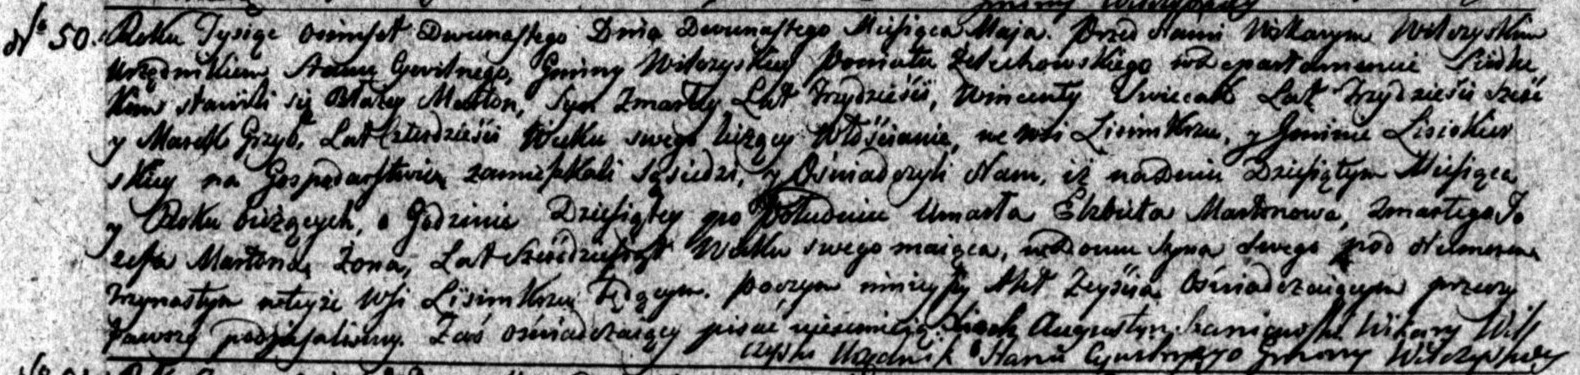
\includegraphics[width=1.0\linewidth]{
        1812_Elżbieta_Marton_Gomoła_akt_zgonu_parafia_Wilczyska_wpis_50.jpg}
    \captionsetup{format=hang}
    \caption{Akt zgonu Elżbiety Marton (z~domu Gomoły) - par. Wilczyska 
    1812~rok (50/1812) \cite{par_wilczyska1}.}
    \label{fig:egomola_1812}
\end{figure}

W~1748~roku w~Dziewulach urodziła się Elżbieta Dziewulska Gomoła, 
córka Wojciecha i~Agnieszki (patrz ryc. \ref{fig:egomola_1748}), czy jest to 
ta sama osoba, która potem w~1783~roku w~Wilczyskach wzięła ślub z Józefem 
Martonem? Nie da się tego stwierdzić z~całkowitą pewnością, dodatkową 
przesłanką uwiarygadniającą tę tezę jest pojawienie się w~akcie chrztu 
z~1785~roku Agnieszki Gomoliny z Wnętrznego (\enquote{...Chrzest: Antoni 
Mendzyński, organista kościoła oraz Agnieszka Gomolina z~Wnętrznego...}), 
która została matką chrzestną Magdaleny Kruk - patrz ryc. 
\ref{fig:gomola2_lubgens}. Agnieszka Gomoła nie została ochrzczona w~parafii 
w~Wilczyskach, nie ma tam też informacji o~jej ślubie, a~zastosowanie w~jej 
przypadku formy nazwiska \enquote{Gomolina} wskazywałoby, iż jest ona 
wdową\footnote{Nazwisko Gomoła / Gomolak / Gomuła w~formie \enquote{Gomolina}
występuje w~aktach~metrykalnych tylko w stosunku do owdowiałych kobiet, tak 
jak nazwisko w formie \enquote{Gomolanka} występuje dla niezamężnych 
panien.}. Być może więc Elżbieta Dziewulska Gomoła przybyła do Wnętrznego 
z~Dziewul wraz ze swoją matką Agnieszką Dziewulską Gomołą, wdową po 
Wojciechu? Pytanie czy inni Gomołowie, którzy pojawili się we~Wnętrznym 
w~podobnym okresie, nie byli braćmi i~siostrami Elżbiety, urodzonymi po 
1750~roku, a~więc nie sposób jest potwierdzić ich chrztu w~Zbuczynie, ze 
względu na brak ksiąg metrykalnych z~tamtej parafii z~lat 1750-1765? Jest to 
prawdopodobne, wskazywać na to może fakt, bliskiego powiązania Gomołów 
przybyłych do Wnętrznego z~rodziną Kruków - Adam Kruk był świadkiem na 
ślubach trzech Gomolaków z~lat 80.~XVIII~wieku: (Antoniego, Kazimierza 
i~Andrzeja), Gomołowie i~Krukowie byli wzajemnie chrzestnymi swoich dzieci, 
zgłaszali zgony członków swojej rodziny\footnote{Co ciekawe, zgodnie 
z~obecnie dostępnymi dokumentami, Gomolakowie z~Wnętrznego nie byli nigdy 
świadkami na ślubach osób o~nazwisku Gomolak, nie byli nawet chrzestnymi 
dzieci o~tym nazwisku. Jedyne silniejsze powiązanie pomiędzy Gomolakami 
z~Wnętrznego, które można odnaleźć w~dokumentach, to powiązanie córek 
Antoniego Gomoły i~Andrzeja Gomoły - Anny (ur. 1800~r. - zm.~?) i~Krystyny 
(ur. 1798~r. - 1842~r.), które przeprowadziły się w~latach 20.~XIX~wieku, do 
oddalonego o~około 50~kilometrów Rudzienka by pracować w~służbie na 
tamtejszym dworze. Co więcej obie wyszły za mąż tego samego dnia - 
29~stycznia 1826~roku, w~parafii pod wezwaniem Świętej Trójcy w~Kołbieli. 
Historia Anny i~Krystyny Gomołów zostanie szerzej opowiedziana w~trzecim 
rozdziale niniejszej książki.}.

\begin{figure}[!ht]
    \vspace*{0.5cm}
    \centering \includegraphics[width=1.0\linewidth]{
        1825_Kazimierz_Gomoła_akt_zgonu1_parafia_Wilczyska_wpis_50.jpg}
    \captionsetup{format=hang}
    \caption{Akt zgonu Kazimierza Gomuły: część~1 - par. Wilczyska 1825~rok 
    (50/1825) \cite{par_wilczyska1}.}
    \label{fig:kgomola1}
\end{figure}

Kontynuując opowieść o~Gomołach zamieszkujących Wnętrzne pod koniec 
XVIII~wieku: dnia 29~maja~1785~roku w~parafii Wilczyska Kazimierz Gomolak 
ożenił się z~Jadwigą Kanią, oboje wywodzili się ze stanu chłopskiego 
i~pochodzili ze wsi Wnętrzne i~tam też w~kolejnych latach rodziły się ich 
dzieci (patrz: ryc. \ref{fig:gomola2_lubgens}). Kazimierz Gomolak 
prawdopodobnie nie urodził się w~parafii Wilczyska, akt chrztu osoby o~takim 
imieniu i~nazwisku nie występuje w~tej parafii, jest więc kolejną osobą 
o~nazwisku Gomoła / Gomolak / Gomuła, która prawdopodobnie sprowadziła się do 
Wnętrznego pod koniec XVIII~wieku. Pierwsza żona Kazimierza Gomolaka, 
Jadwiga, zmarła w~1796~roku, 11~lat po ich ślubie. Rok później w~1797~roku 
Kazimierz wziął kolejny ślub tym razem z~Antoniną Makolówną (patrz: ryc. 
\ref{fig:gomola2_lubgens}). Z~aktu zgonu Kazimierza Gomuły z~1825~roku 
wynika, iż w~momencie śmierci miał on około 63~lata, co oznacza, iż urodził 
się on około 1762~roku (patrz: ryc. \ref{fig:kgomola2}). Ostatnią osobą, 
która pojawiła się we Wnętrznym w~latach 80.~XVIII~wieku i~nosiła nazwisko 
Gomoła / Gomolak / Gomuła, był Andrzej Gomolak. Dnia 4~lutego 1787~roku wziął 
on ślub z~Agatą Pieniak pochodzącą z~sąsiedniej wsi Gródź (patrz: ryc. 
\ref{fig:gomola2_lubgens}) - jak wskazuje wpis w~bazie indeksów metrykalnych 
\emph{Lubgens} dotyczący ich ślubu, oboje należeli do stanu chłopskiego. 
Podobnie jak w~przypadku pozostałych Gomolaków, tak również w~przypadku 
Andrzeja, w~parafii Wilczyska nie występuje akt jego chrztu, a~przynajmniej 
nie ma o~nim wzmianki w~bazie \emph{Lubgens} przed 1787~rokiem. W~bazie tej 
występuje natomiast informacja, iż, Andrzej Gomoła, ojciec rodziny, zmarł 
w~1801~roku, w~wieku 36~lat, z~powodu apopleksji - oznacza to, iż urodził się 
on około 1765~roku (patrz: ryc. \ref{fig:gomola2_lubgens}).

\begin{figure}[!ht]
    \vspace*{0.5cm}
    \centering \includegraphics[width=1.0\linewidth]{
        1825_Kazimierz_Gomoła_akt_zgonu2_parafia_Wilczyska_wpis_50.jpg}
    \captionsetup{format=hang}
    \caption{Akt zgonu Kazimierza Gomuły: część~2 - par. Wilczyska 1825~rok 
    (50/1825) \cite{par_wilczyska1}.}
    \label{fig:kgomola2}
\end{figure}

Mamy więc finalnie osiem osób zamieszkałych we Wnętrznym, należących do stanu 
chłopskiego, których nazwiska Gomoła / Gomolak / Gomuła pojawiają się 
w~aktach metrykalnych parafii Wilczyska z~końcówki XVIII~wieku, a~którzy, jak 
wszystko na to wskazuje, nie urodzili się na terenie wilczyńskiej parafii:

\begin{itemize}
    \item Jadwiga Gomulicha (ur. ok. 1730~r. - zm. 1812~r.),
    \item Maciej Gomolak (ur.~? - zm. 1779~r.)
    \item \textbf{Antoni Gomolak} (ur. ok. 1764~r. - zm. 1810~r.),
    \item Piotr Gomolak (ur. ok. 1750~r. - zm. 1821~r.),
    \item Elżbieta Gomolanka (ur. ok. 1750~r. - zm. 1812~r.),
    \item Agnieszka Gomolina (ur.~? - zm.~?),
    \item Kazimierz Gomlak (ur. ok. 1762~r. - zm. 1825~r.),
    \item Andrzej Gomolak (ur. ok. 1765~r. - zm. 1801~r.). 
  \end{itemize}

W~świetle dostępnych obecnie dokumentów, nie można jednoznacznie stwierdzić, 
skąd wyżej wymienione osoby przybyły do Wnętrznego ani jakie były między nimi 
powiązania rodzinne. \textbf{Najbardziej prawdopodobna wydaje się hipoteza, 
iż Gomolakowie zamieszkujący wieś Wnętrzne w~końcówce XVIII~wieku przybyli 
tam z~Dziewul}, w~procesie ubożenia stracili ziemię, status szlachty 
i~nazwisko Dziewulski, związane z~rodzinną miejscowością, a~po przeprowadzce 
do Wnętrznego stali się zwykłymi najemnymi chłopami. Na taki scenariusz 
wskazywałyby następujące przesłanki:

\begin{itemize}
    \item nagłe pojawienie się Gomolaków we Wnętrznym, w~sytuacji 
    równoczesnego zanikania w~Dziewulach gałęzi Dziewulskich posługującej się 
    przydomkami Gomolak / Gomolik / Gomoła / Gomuła,
    \item zbieżność imion i~dat urodzenia niektórych członków rodziny 
    Gomolaków z~odpowiadającym im Dziewulskim (Jadwiga, Maciej, Elżbieta, 
    Agnieszka),
    \item posługiwanie się przez Gomolaków z~Wnętrznego trzema z~czterech 
    charakterystycznych przydomków dla jednej z~gałęzi Dziewulskich 
    (Gomolak / Gomoła / Gomuła),
    \item fakt, iż w~żadnej z~okolicznych parafii, poza Zbuczynem, nazwiska 
    Gomoła / Gomolak / Gomuła nie występowały powszechnie.
\end{itemize}
 
Ciągnąc dalej tę hipotezę można stwierdzić, iż Gomołowie najprawdopodobniej 
przybyli do Wnętrznego jako trzy rodziny:

\begin{enumerate}
    \item Rodzina Tomasza Gomolaka, który przybył do Wnętrznego około 
    1714~roku - z~lini tej wywodzą się Gomołowie, którzy do dnia dzisiejszego 
    mieszkają w~Woli Mysłowskiej.
    \item Rodzina Macieja Gomolaka i~Jadwigi Gomulichy, którzy przybyli do 
    Wnętrznego około 1765~roku - linia ta wygasła ze wzgledu na brak 
    męskich potomków.
    \item Rodzina Wojciecha i~Agnieszki Gomolaków, którzy przybyli do 
    Wnętrznego w~latach 70.~XVIII wieku razem z~dziećmi: Elżbietą, Piotrem,
    Kazimierzem, Antonim i~Andrzejem - z~linii tej wywodzą się Gomołowie, 
    którzy do dnia dzisiejszego zamieszkują Mysłów oraz Gomulscy 
    zamieszkujący obecnie okolice Mińska Mazowieckiego.
\end{enumerate}

Nie da się w~pełni zweryfikować wyżej postawionych hipotez bez dostępu do 
pełnych akt metrykalnych z~XVIII~wieku dla parafii pod wezwaniem św. 
Stanisława Biskupa Męczennika i~Aniołów Stróżów w~Zbuczynie oraz parafii pod 
wezwaniem Niepokalanego Serca Najświętszej Maryi Panny w~Wilczyskach. Być może 
dostęp do tych akt będzie możliwy w~przyszłości i~uda się zweryfikować chociaż 
część z~wyżej postawionych hipotez w~kolejnym wydaniu niniejszej książki.

% Przednia okładka podrozdziału
\clearpage
\includepdf{Mysłów_mapa_fin.png}

\section{Mysłów: 1783~r. - 1810~r.}

Wieś Mysłów w~XVIII~wieku znajdowała się na granicy województw lubelskiego, 
mazowieckiego i~sandomierskiego, zaliczana była do ziemi łukowskiej. 
Najbliższymi dużymi ośrodkami miejskimi dla Mysłowa były: oddalony 
o~około 35~kilometrów na wschód Łuków oraz oddalony o~około 30~kilometrów na 
zachód Garwolin. Wieś ta należała w~tamtym czasie do parafii 
rzymskokatolickiej pod wezwaniem Niepokalanego Serca Najświętszej Maryi Panny 
w~Wilczyskach. Mysłów został założony prawdopodobnie około 1531~roku - wynika 
to zapisów rejestrów poborowych województwa lubelskiego \cite{apawinski} 
(patrz: ryc. \ref{fig:wilczyska_1531}). W~XVI~wieku właścicielami Mysłowa 
była rodzina Mysłowskich, jednak pod koniec XVIII wieku wieś ta stanowiła 
część pokaźnego majątku rodziny Rzewuskich (herbu Krzywda), a~konkretnie jej 
właścicielem był Tomasz Rzewuski, chorąży łukowski. \nocite{sulimierski}

\begin{figure}[!ht]
    \vspace*{0.5cm}
    \centering 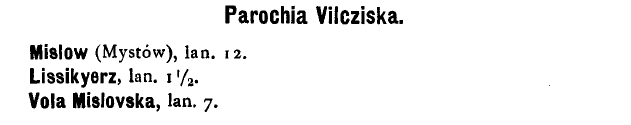
\includegraphics[width=0.9\linewidth]{Wilczyska_1531.png}
    \captionsetup{format=hang}
    \caption{Wpis dotyczący parafii Wilczyska pochodzący z~rejestrów 
    poborowych województwa lubelskiego z~1531~roku \cite{apawinski}.}
    \label{fig:wilczyska_1531}
\end{figure}

Dnia 16~lutego 1783~roku około dziewiętnastoletni Antoni Gomoła poślubił 
w~Wilczyskach około piętnastoletnią \textbf{Petronellę Sokół}, urodzoną 
prawdopodobnie w~1768~roku w~Mysłowie. Z~ich małżeństwa narodziło 
dziewięcioro dzieci: 

\begin{itemize}
  \item Mariana (ur. 1783~r. - zm. 1803~r.),
  \item Franciszka (ur. 1785~r. - zm. 1803~r.),
  \item Wojciech (ur. 1787~r. - zm. 1847~r.),
  \item \textbf{Jan} (ur. 1789~r. - zm. 1851~r.),
  \item Katarzyna (ur. 1791~r. - zm. 1800~r.),
  \item Salomea (ur. 1792~r. - zm. 1794~r.),
  \item Tadeusz (ur. 1794~r. - zm. 1828~r.),
  \item Józefa (ur. 1798~r. - zm. 1799~r.),
  \item Anna (ur. 1800~r. - zm.~?).
\end{itemize}

Z~dziewięciorga dzieci Petronelli i~Antoniego własne rodziny założyła tylko 
czwórka: najstarszy syn Wojciech, jego młodszy brat Jan, najmłodszy syn 
Tadeusz oraz najmłodsza córka Anna - pięć pozostałych córek zmarło, albo 
w~bardzo młodym wieku, albo z~powodu chorób zakaźnych.

\begin{figure}[!ht]
    \vspace*{0.5cm}
    \centering 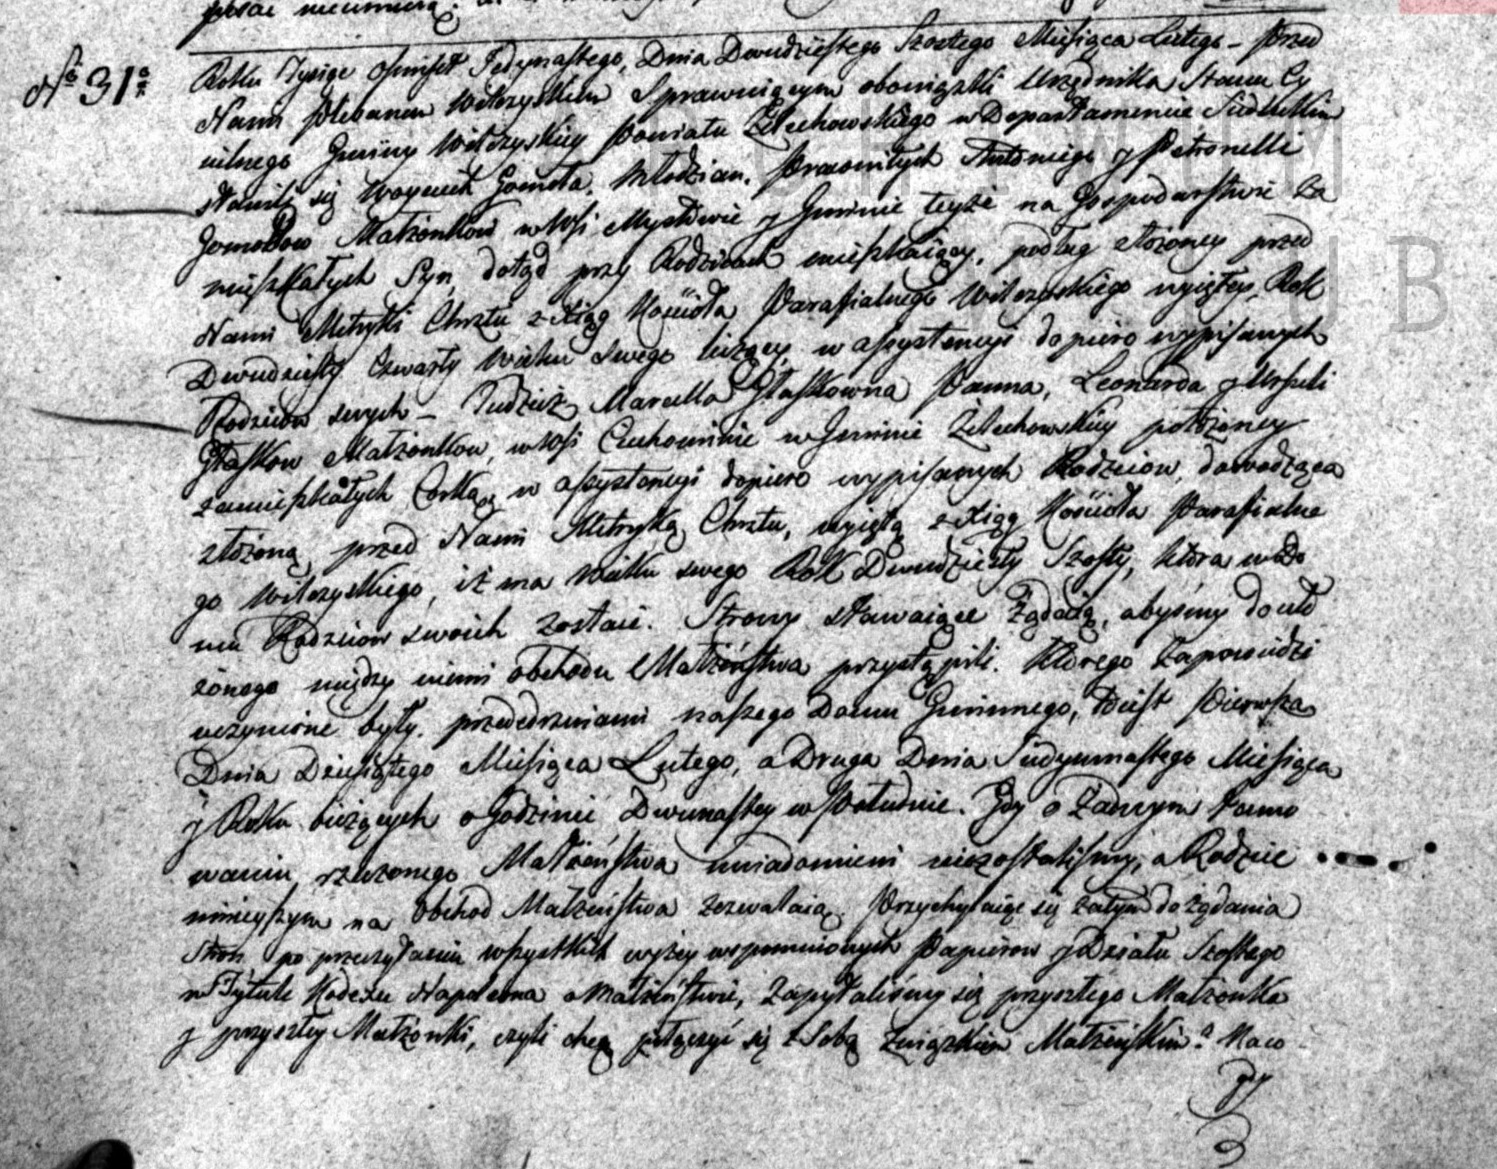
\includegraphics[width=1.0\linewidth]{
        1811_Wojciech_Gomoła_Marcella_Głasek_akt_ślubu1_parafia_Wilczyska_wpis_31.jpg}
    \captionsetup{format=hang}
    \caption{Akt ślubu Wojciecha Gomoły i~Marcelli Głasek część~1 - par. 
    Wilczyska 1811~rok (31/1811) \cite{par_wilczyska1}.}
    \label{fig:wmgomola_slub1}
\end{figure}

\begin{figure}[!ht]
    \vspace*{0.5cm}
    \centering 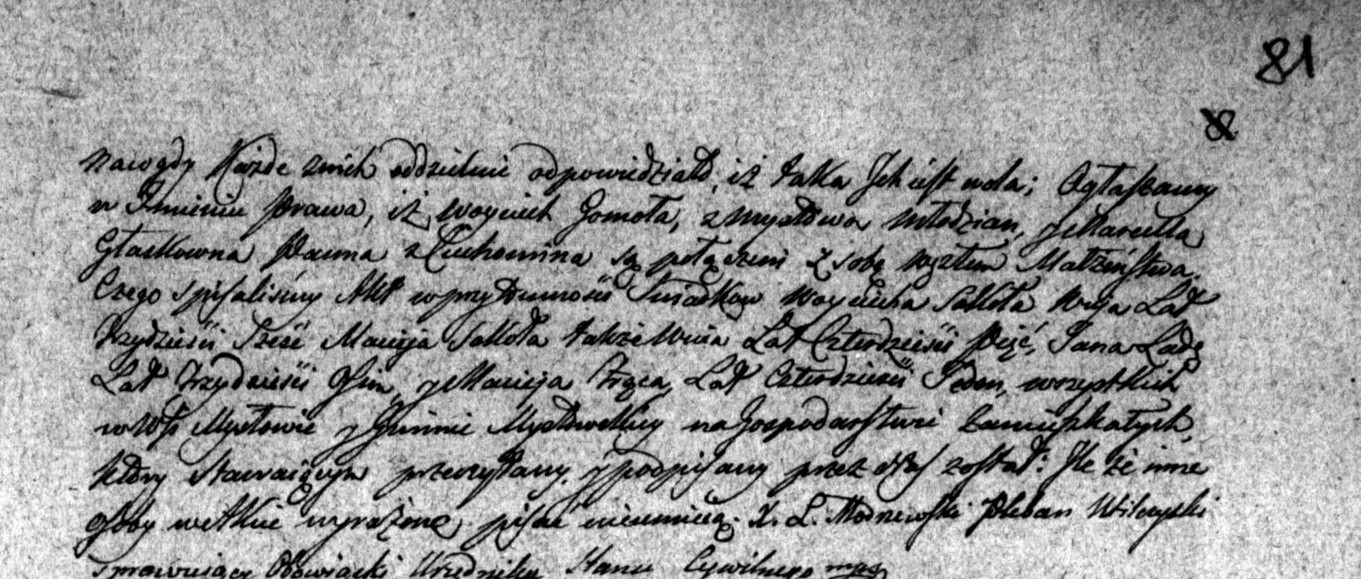
\includegraphics[width=1.0\linewidth]{
        1811_Wojciech_Gomoła_Marcella_Głasek_akt_ślubu2_parafia_Wilczyska_wpis_31.jpg}
    \captionsetup{format=hang}
    \caption{Akt ślubu Wojciecha Gomoły i~Marcelli Głasek część~2 - par. 
    Wilczyska 1811~rok (31/1811) \cite{par_wilczyska1}.}
    \label{fig:wmgomola_slub2}
\end{figure}

Dwie najstarsze córki Antoniego i~Petronelli Gomołów, Marianna i~Franciszka, 
obie już pełnoletnie, w~wieku 19~i~18~lat, zmarły z~powodu gorączki 
suchotniczej. Trzy lata przed ich śmiercią, w~1800~roku, z~powodu gorączki 
suchotniczej zmarła ich dziewięcioletnia siostra Katarzyna, rok przed tym, 
ospa doprowadziła do śmierci ich kilkumiesięcznej siostry Józefy (mylnie 
nazwanej w~bazie indeksów metrykalnych \emph{Lubgens}, we wpisie dotyczącym 
jej zgonu, Marianną), a~sześć lat wcześniej, w~1794~roku, zmarła mająca 
zaledwie rok Salomea (patrz: ryc. \ref{fig:gomola3_lubgens}).

\begin{figure}[!ht]
    \vspace*{0.5cm}
    \centering 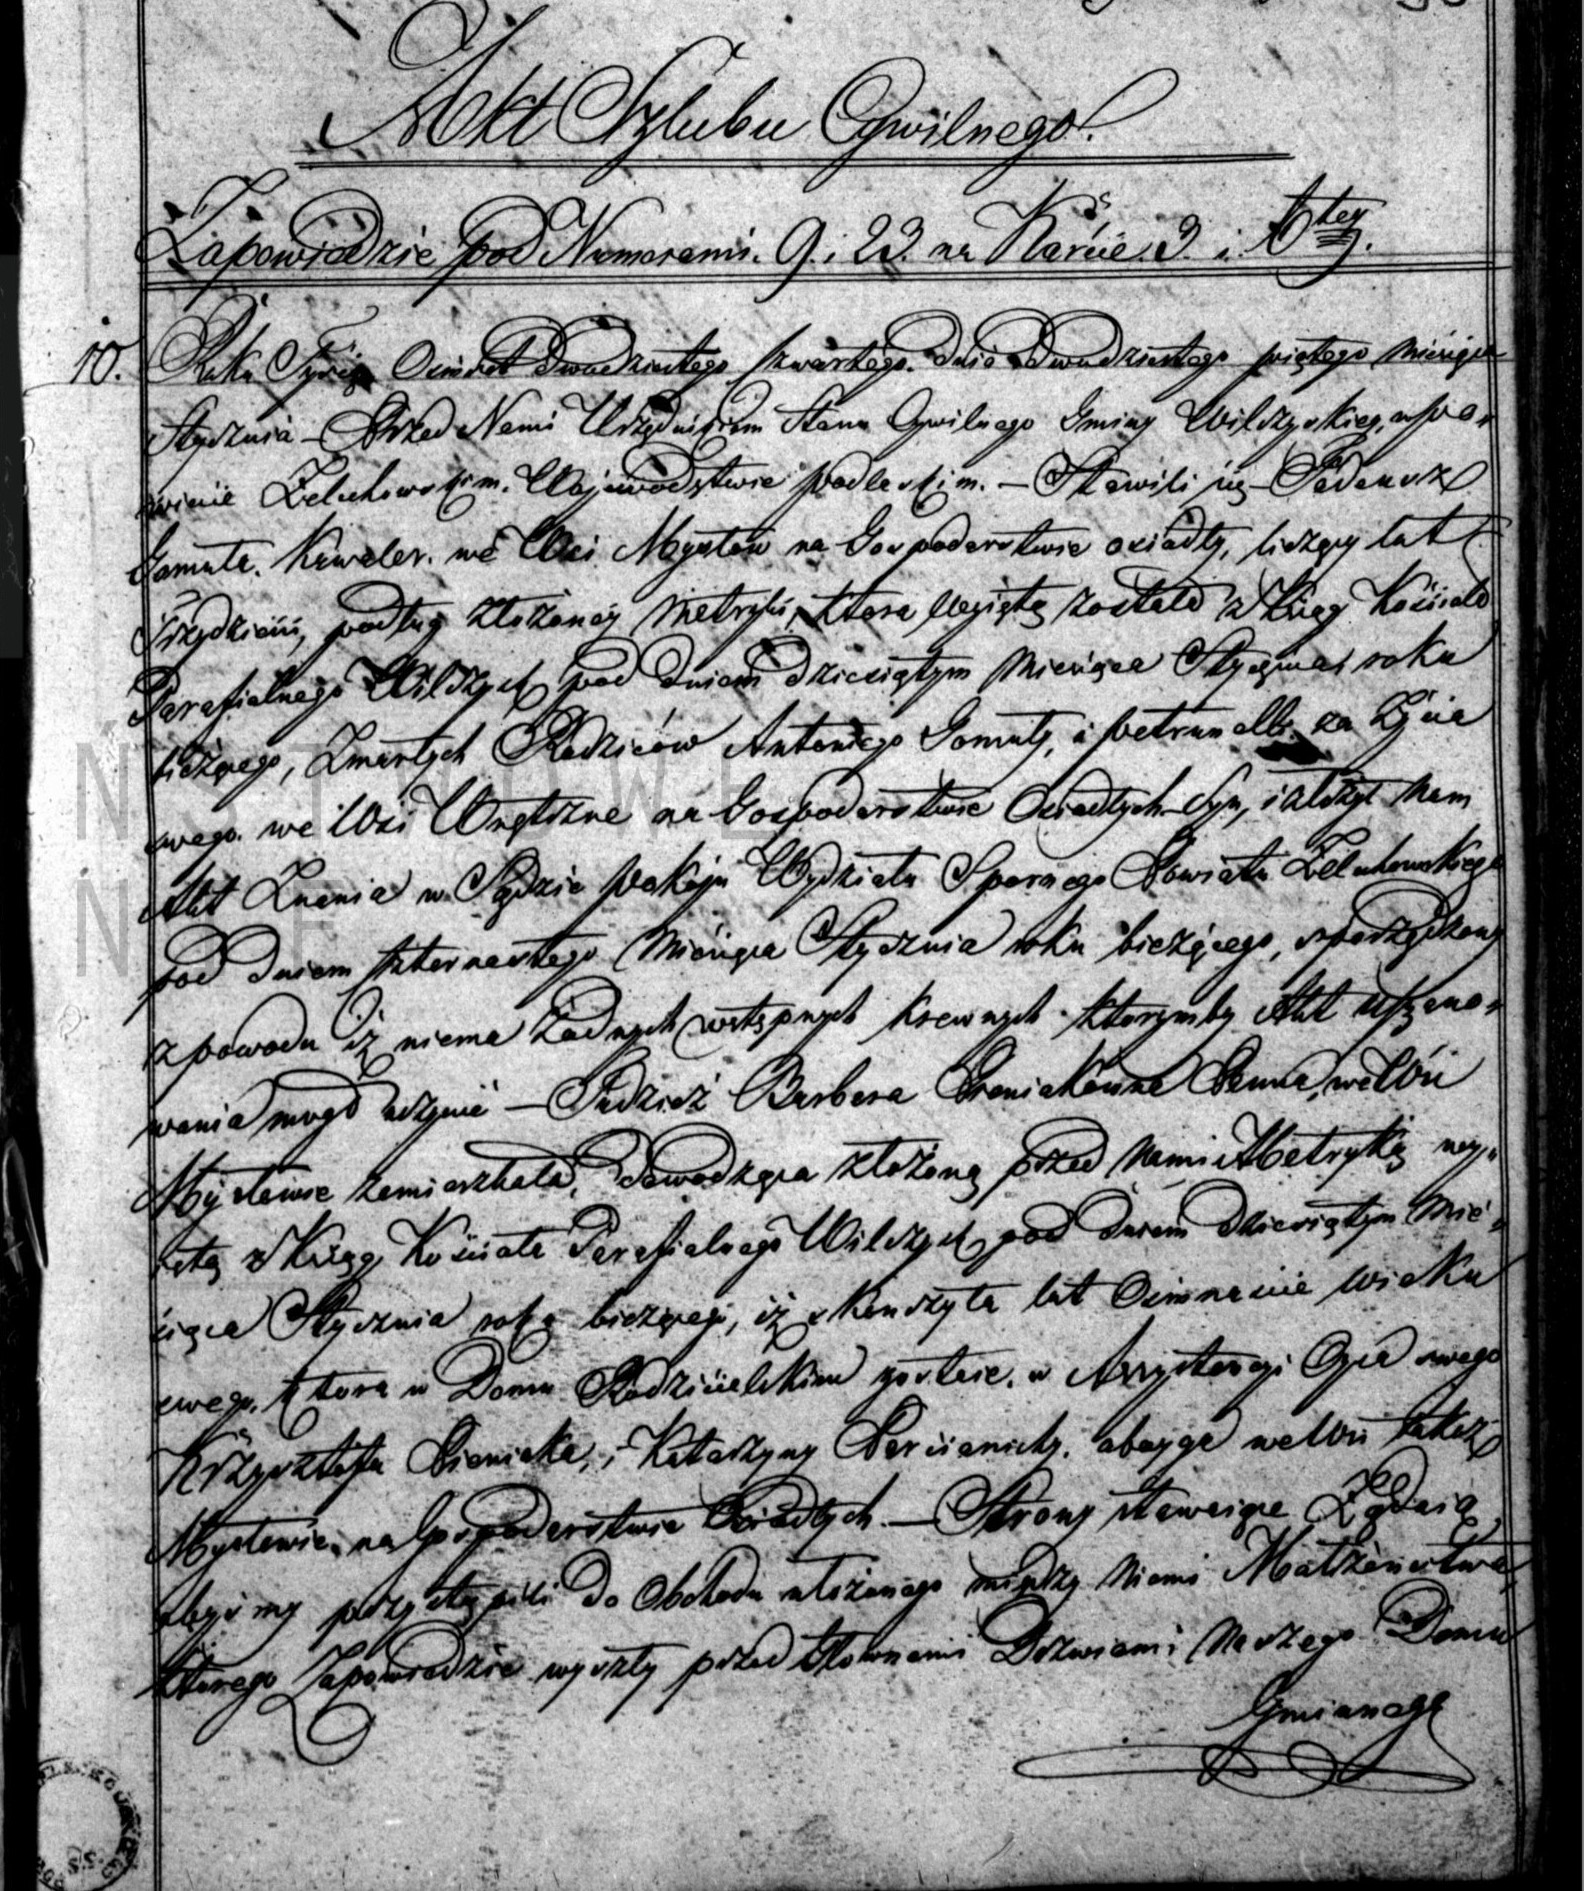
\includegraphics[width=0.95\linewidth]{
        1824_Tadeusz_Gomuła_Barbara_Pieniak_akt_ślubu_parafia_Wilczyska_wpis_10.jpg}
    \captionsetup{format=hang}
    \caption{Akt ślubu Tadeusza Gomoły i~Barbary Pieniak - par. Wilczyska 
    1824~rok (10/1824) \cite{par_wilczyska1}.}
    \label{fig:tbgomola_slub}
\end{figure}

\begin{figure}[!ht]
    \vspace*{0.5cm}
    \centering 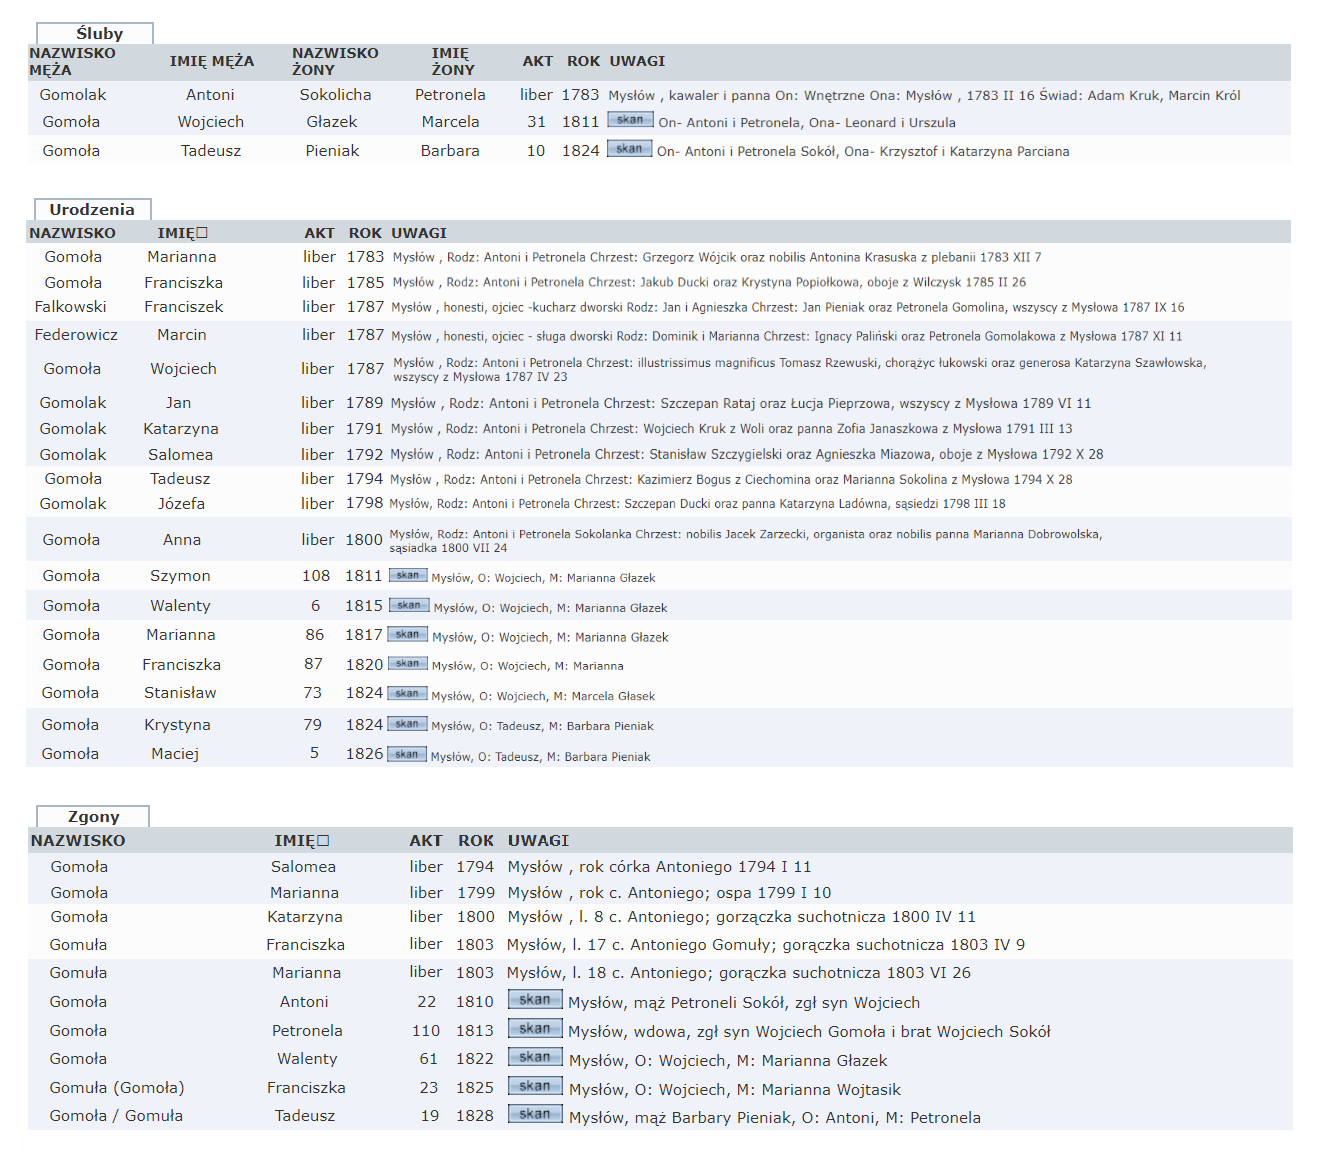
\includegraphics[width=1.0\linewidth]{
        Gomołowie_Mysłów_wpisy_Lubgens.png}
    \captionsetup{format=hang}
    \caption{Wpisy w~bazie indeksów metrykalnych \emph{Lubgens} dotyczące 
    Gomołów, którzy mieszkali we wsi Mysłów na przełomie XVIII~i~XIX~wieku.}
    \label{fig:gomola3_lubgens}
\end{figure}

Antoni i~Petronella Gomołowie byli prawdopodobnie silnie związani z~dworem 
w~Mysłowie, być może w~pewnym okresie pracowali tam jako służący lub chłopi 
najemni, świadczyć o~tym może fakt, iż Petronella została matką chrzestną 
syna kucharza dworskiego Franciszka Falkowskiego oraz syna służącego 
dworskiego Marcina Federowicza (patrz: ryc. \ref{fig:gomola3_lubgens}). Co 
więcej, ojcem chrzestnym najstarszego syna Antoniego i~Petronelli, Wojciecha, 
został Tomasz Rzewuski, chorąży łukowski, jedyny dziedzic pokaźnego majątku 
Rzewuskich, w~skład którego, w~tamtych latach, wchodził m.in. dwór 
w~Mysłowie, wieś Mysłów oraz liczne okoliczne wsie (patrz: ryc. 
\ref{fig:gomola3_lubgens}). Wojciech Gomoła był jedyną osobą w~parafii 
Wilczyska, zgodnie z~zapisami bazy \emph{Lubgens}, którego chrzestnym ojcem 
został Tomasz Rzewuski, mimo iż do tej parafii należały liczne dwory m.in 
dwór w~Ciechominie, dwór w~Wilczyskach, dwór w~Jarczewie, dwór w~Goniwilku, 
dwór w~Woli Mysłowskiej, dwór w~Kamieniu, dwór w~Lisikierzu czy dwór we 
Wnętrznym, na których rodziły się dzieci osób wywodzacych się ze znamienitych 
rodów szlacheckich takich jak: ród Orsettich, ród Sikorskich, ród Ostrorogów, 
ród Rostworowskich, czy ród Przegalińskich. Fakt, iż ojcem chrzestnym 
Wojciecha Gomoły, został Tomasz Rzewuski, musiał być więc dużym wyróżnieniem 
dla całej rodziny Gomołów z~Mysłowa (należących, według zapisów w~bazie 
indeksów metrykalnych \emph{Lubgens}, do stanu chłopskiego) - fakt ten może 
równieżwzmacniać hipotezą o~szlacheckich korzeniach rodziny Gomołów. 

\begin{figure}[!ht]
    \vspace*{0.5cm}
    \centering 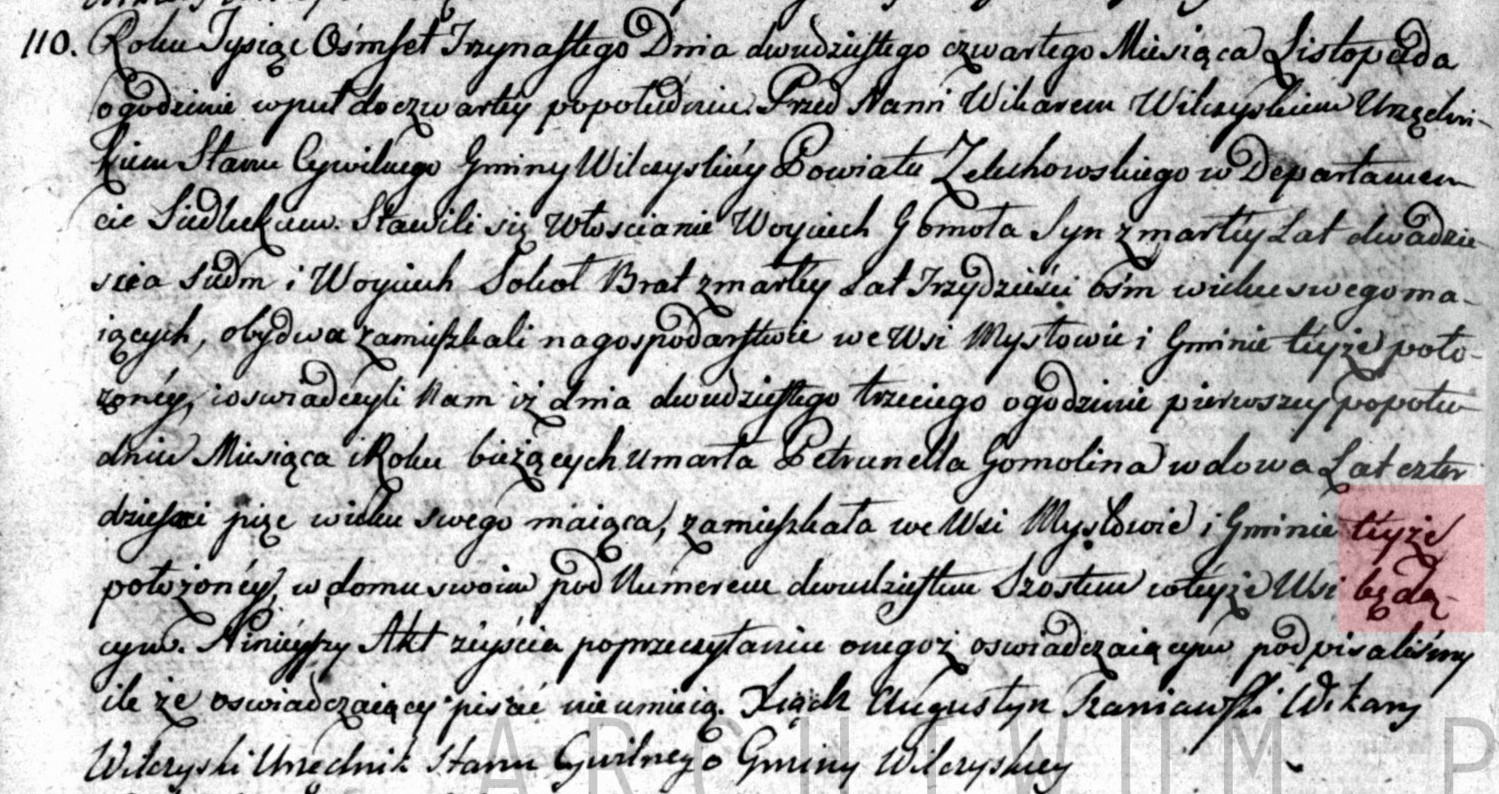
\includegraphics[width=1.0\linewidth]{
        1813_Petronella_Gomoła_Sokół_akt_zgonu_parafia_Wilczyska_wpis_110.jpg}
    \captionsetup{format=hang}
    \caption{Akt zgonu Petronelli Gomoły (z~domu Sokół) - par. Wilczyska 
    1813~rok (110/1813) \cite{par_wilczyska1}.}
    \label{fig:pgomola_1813}
\end{figure}

\begin{figure}[!ht]
    \vspace*{0.5cm}
    \centering \includegraphics[width=1.0\linewidth]{
        1828_Tadeusz_Gomuła_akt_zgonu_parafia_Wilczyska_wpis_19.jpg}   
    \captionsetup{format=hang}
    \caption{Akt zgonu Tadeusza Gomoły - par. Wilczyska 1828~rok (19/1828) 
    \cite{par_wilczyska1}.}
    \label{fig:tgomola_1828}
\end{figure}

Petronella i~Antoni Gomołowie resztę swojego życia, od momentu ślubu, 
spędzili najprawdopodobniej w~Mysłowie. Antoni zmarł 22~grudnia 1810~roku, 
w~wieku około 46~lat (patrz: ryc. \ref{fig:agomola}), a~jego żona Petronella, 
trzy lata później - 23~listopada 1813~roku w~wieku około 45~lat  (patrz: ryc. 
\ref{fig:pgomola_1813}). Ich potomkowie o~nazwisku Gomoła mieszkają po dzień 
dzisiejszy w~Mysłowie - jest to gałąź rodziny wywodząca się od ich 
najstarszego syna Wojciecha, który wraz z~żoną Marcellą oraz piątką dzieci 
osiadł w~rodzinnej wsi swojej matki. Młodszy brat Wojciecha Jan, w~wieku 
około dwudziestu lat, przeprowadził się do oddalonego o~50~kilometrów na 
północny zachód Rudzienka, gdzie stał się założycielem rodziny Gomulskich 
zamieszkującej do dnia dzisiejszego okolice Mińska Mazowieckiego. Natomiast 
potomkowie najmłodszego z~braci Gomołów, Tadeusza, związali swe losy 
z~pobliską Wolą Mysłowską.

\begin{figure}[!ht]
    \vspace*{0.5cm}
    \centering 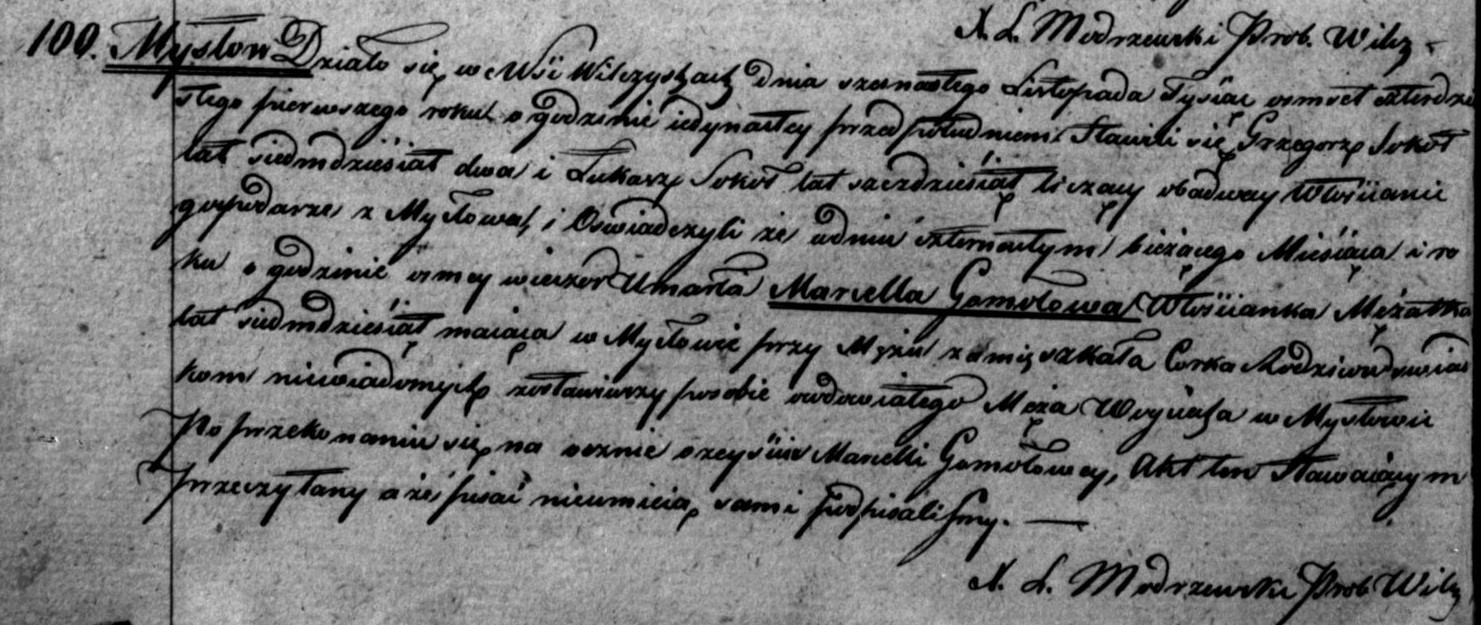
\includegraphics[width=1.0\linewidth]{
        1841_Marcella_Gomoła_Głasek_akt_zgonu_parafia_Wilczyska_wpis_100.jpg}  
    \captionsetup{format=hang}
    \caption{Akt zgonu Marcelli Gomoły (z~domu Głasek) - par. Wilczyska 
    1841~rok (100/1841) \cite{par_wilczyska1}.}
    \label{fig:mgomola_1841}
\end{figure}

\begin{figure}[!ht]
    \vspace*{0.5cm}
    \centering \includegraphics[width=1.0\linewidth]{
        1847_Wojciech_Gomoła_akt_zgonu_parafia_Wilczyska_wpis_66.jpg}    
    \captionsetup{format=hang}
    \caption{Akt zgonu Wojciecha Gomoły - par. Wilczyska 1847~rok (66/1847) 
    \cite{par_wilczyska1}.}
    \label{fig:wgomola_1847}
\end{figure}

Petronella Sokół pochodziła z~licznej w~tamtym czasie w~Mysłowie rodziny 
Sokołów, zamieszkującej tę wieś conajmniej od połowy XVII~wieku. Jej 
rodzicami byli prawdopodobnie\footnote{Nie możemy być całkowicie pewni, że 
Andrzej i~Agnieszka Sokołowie, byli rodzicami Petronelli Gomoły, gdyż w~bazie 
indeksów metrykalnych \emph{Lubgens} nie ma wpisu dotyczącego jej chrztu. 
Jest to jednak wysoce prawdopodobne analizując jej akt zgonu oraz akt zgonu 
Macieja Sokoła.} Andrzej (ur. 1728~r. - zm. 1807~r.) oraz Agnieszka (ur. 
1735~r. - zm. 1804~r.), z~domu Nowak. Andrzej i~Agnieszka Sokołowie, poza 
córką Petronellą, posiadali jeszcze co najmniej ósemkę dzieci: 

\begin{itemize}
  \item Józefa (ur. 1756~r. - zm.~?),
  \item Mariannę (ur. 1758~r.  - zm. 1825~r.),
  \item Urszulę (ur. 1760~r. - zm.~?),
  \item Magdalenę (ur. 1763~r. - zm.~?),
  \item Macieja (ur. 1766~r. - zm. 1814~r.),
  \item Antoniego (ur. 1769~r. - zm. 1811~r.),
  \item Pawła (ur. 1772~r. - zm.~?),
  \item Wojciecha (ur. 1776~r. - zm. 1827~r.).
\end{itemize}

Wojciech Sokół był świadkiem w~akcie zgonu zarówno Macieja Sokoła (patrz: 
ryc. \ref{fig:msokol_1814}), jak i~Petronelli Gomoły (patrz: ryc. 
\ref{fig:pgomola_1813}), w~obu tych aktach był wymieniony jako 38-letni brat 
zmarłych. Pokrewieństwo Macieja Sokoła i~Petronelli Gomoły jest o~tyle ważne, 
iż syn Macieja Paweł razem z~córką Antoniego i~Petronelli Gomołów 
Anną oraz córką Andrzeja i~Agaty Gomołów z~Wnętrznego (opisywanych 
w~poprzednim podrozdziale) Krystyną, w~latach dwudziestych XIX~wieku, 
przeprowadzili się do Rudzienka, gdzie pracowali w~służbie na tamtejszym 
dworze.

\begin{figure}[!ht]
    \vspace*{0.5cm}
    \centering 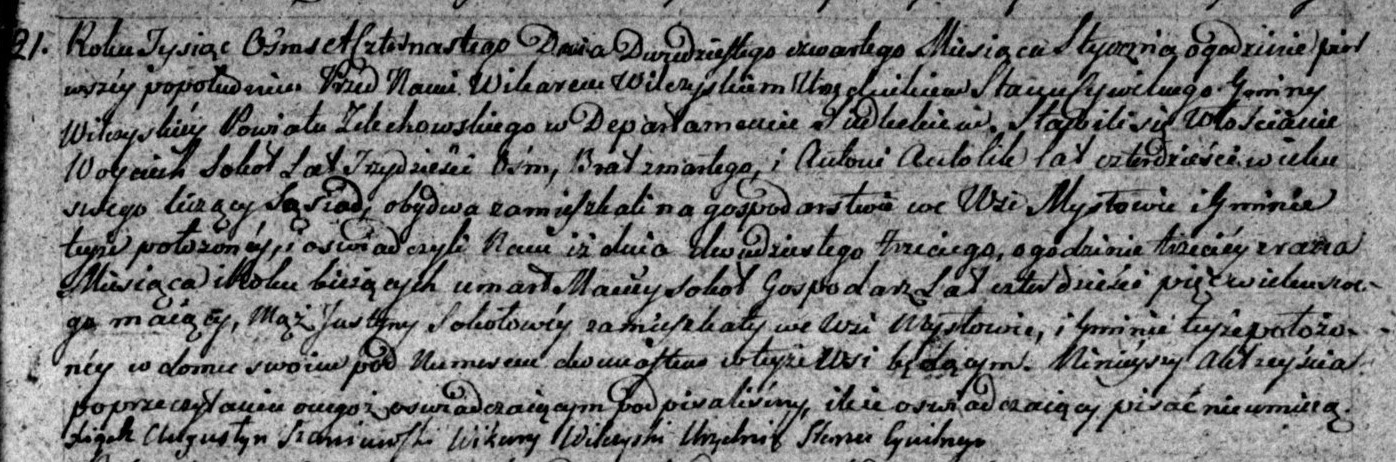
\includegraphics[width=1.0\linewidth]{
        1814_Maciej_Sokół_akt_zgonu_parafia_Wilczyska_wpis_21.jpg}
    \captionsetup{format=hang}
    \caption{Akt zgonu Macieja Sokoła - par. Wilczyska 1814~rok (21/1814) 
    \cite{par_wilczyska1}.}
    \label{fig:msokol_1814}
\end{figure}

Zanim jednak Paweł Sokół, Anna Gomoła oraz Krystyna Gomoła dotarli do 
Rudzienka, około 1810~roku przeprowadził się tam starszy brat Anny Jan, 
który został tam kowalem. \textbf{Jana Gomołę można uznać za założyciela 
rodziny Gomulskich}, jako pierwszy nosił to nazwisko, choć posługiwał się też 
nazwiskiem swojej matki - Sokół, zwany był też Gumułą, Gumulskim, a~w~jego 
akcie zgonu wpisano nazwisko Gromulski. Jego życie wydaje się dosyć 
ekstraordynaryjne jak na dziewiętnastowiecznego chłopa pochodzącego z~małej 
lubelskiej wsi - posługiwał się kilkoma nazwiskami, mieszkał w~pięciu
różnych miejscowościach oddalonych od siebie często o~kilkadziesiąt 
kilometrów, w~czterech różnych parafiach, a~swoim trzem najstarszym synom 
nadał to samo imię - Franciszek (choć dla pierwszego syna Piotra, imię 
Franciszek było drugim imieniem). \textbf{Jan Gomoła vel Sokół vel Gumuła vel 
Gumulski vel Gomulski vel Gromulski} urodził się w~1789~roku w~Mysłowie, 
w~wieku około dwudziestu lat przeprowadził się do oddalonego o~około 
50~kilometrów Rudzienka, gdzie pracował jako kowal. W~wieku 25~lat ożenił się 
z~córką karbowego lokalnego folwarku Łucją Rokicką, następnie wraz z~nią 
i~synem Piotrem Franciszkiem przeprowadził się do Zamienia, potem do 
Grzebowilka, a~swojego żywota dokonał w~miejscowości Stara Wieś (koło 
Siennicy) jako \enquote{były kowal na teraz z~jałmużny się utrzymujący}.

\clearpage
\textbf{\large Podsumowanie najważniejszych informacji o~członkach rodziny 
Gomołów z~Mysłowa}

\begin{figure}[!ht]
    \vspace*{0.5cm}
    \centering \includegraphics[width=0.85\linewidth]{Antoni_Gomoła_karta.png}
\end{figure}

\begin{figure}[!ht]
    \vspace*{0.5cm}
    \centering \includegraphics[width=0.85\linewidth]{
        Petronella_Gomoła_karta.png}
\end{figure}

\begin{figure}[!ht]
    \vspace*{0.5cm}
    \centering \includegraphics[width=0.65\linewidth]{
        Marianna_Gomoła_karta.png}
\end{figure}

\begin{figure}[!ht]
    \vspace*{0.5cm}
    \centering \includegraphics[width=0.65\linewidth]{
        Franciszka_Gomoła_karta.png}
\end{figure}

\begin{figure}[!ht]
    \vspace*{0.5cm}
    \centering \includegraphics[width=0.65\linewidth]{
        Wojciech_Gomoła_karta.png}
\end{figure}

\begin{figure}[!ht]
    \vspace*{0.5cm}
    \centering \includegraphics[width=0.65\linewidth]{
        Marcella_Gomoła_karta.png}
\end{figure}

\begin{figure}[!ht]
    \vspace*{0.5cm}
    \centering \includegraphics[width=0.65\linewidth]{
        Katarzyna_Gomoła_karta.png}
\end{figure}

\begin{figure}[!ht]
    \vspace*{0.5cm}
    \centering \includegraphics[width=0.65\linewidth]{
        Salomea_Gomoła_karta.png}
\end{figure}

\begin{figure}[!ht]
    \vspace*{0.5cm}
    \centering \includegraphics[width=0.65\linewidth]{
        Tadeusz_Gomoła_karta.png}
\end{figure}

\begin{figure}[!ht]
    \vspace*{0.5cm}
    \centering \includegraphics[width=0.65\linewidth]{
        Barbara_Gomoła_karta.png}
\end{figure}

\begin{figure}[!ht]
    \vspace*{0.5cm}
    \centering 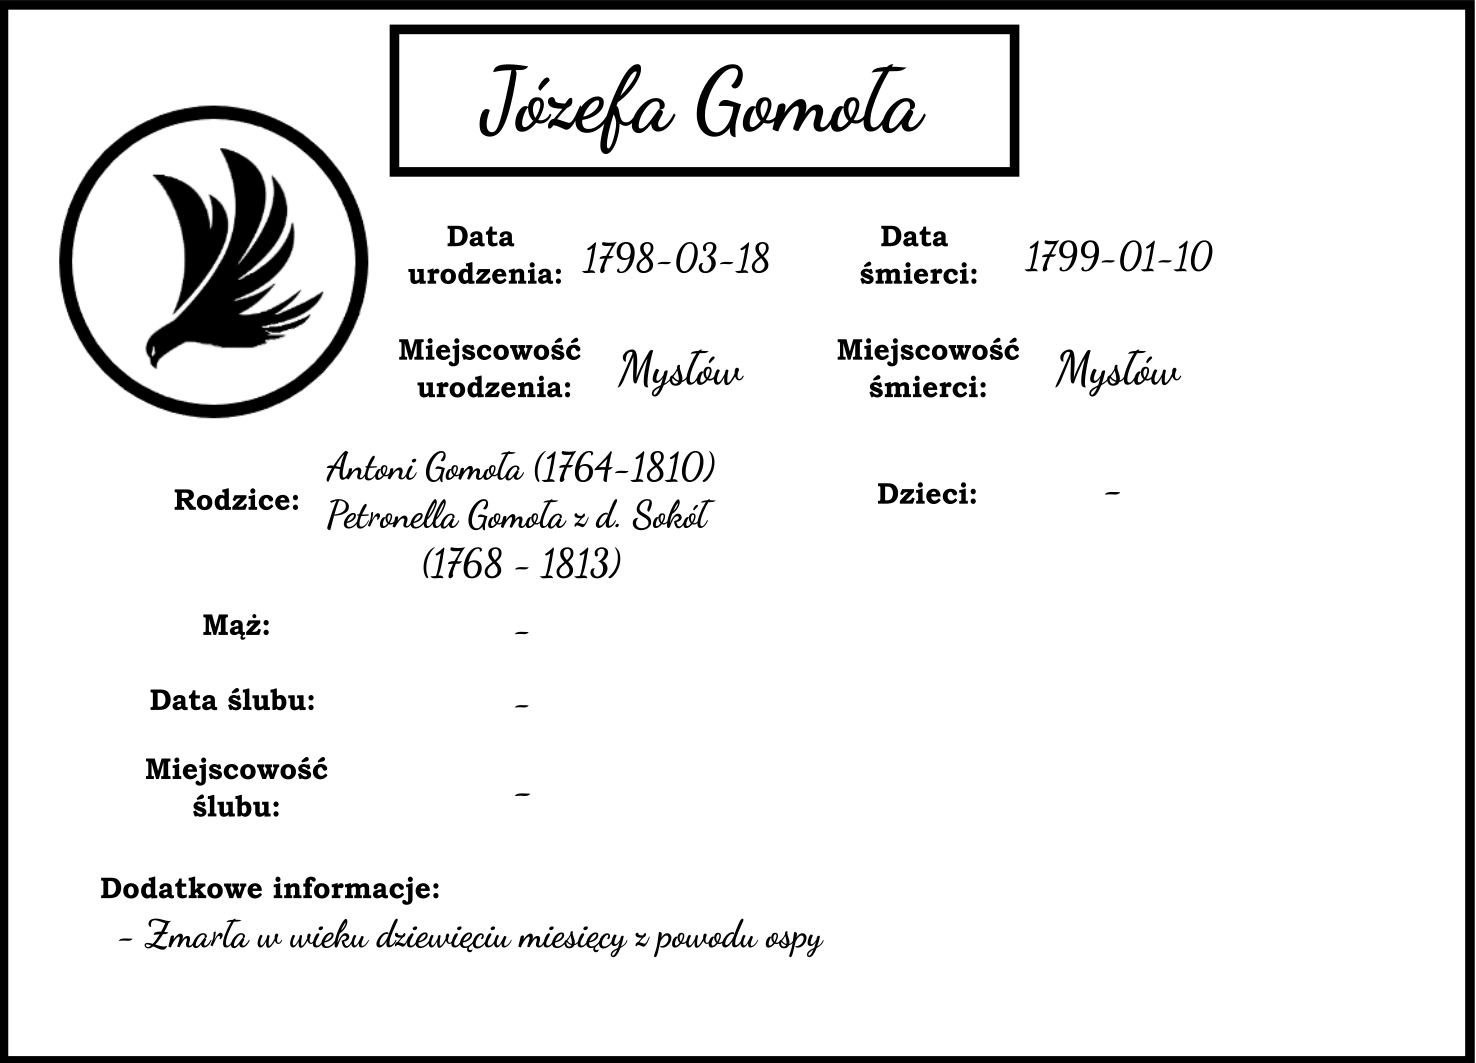
\includegraphics[width=0.65\linewidth]{
        Józefa_Gomoła_karta.png}
\end{figure}

\begin{sidewaysfigure}
    \centering 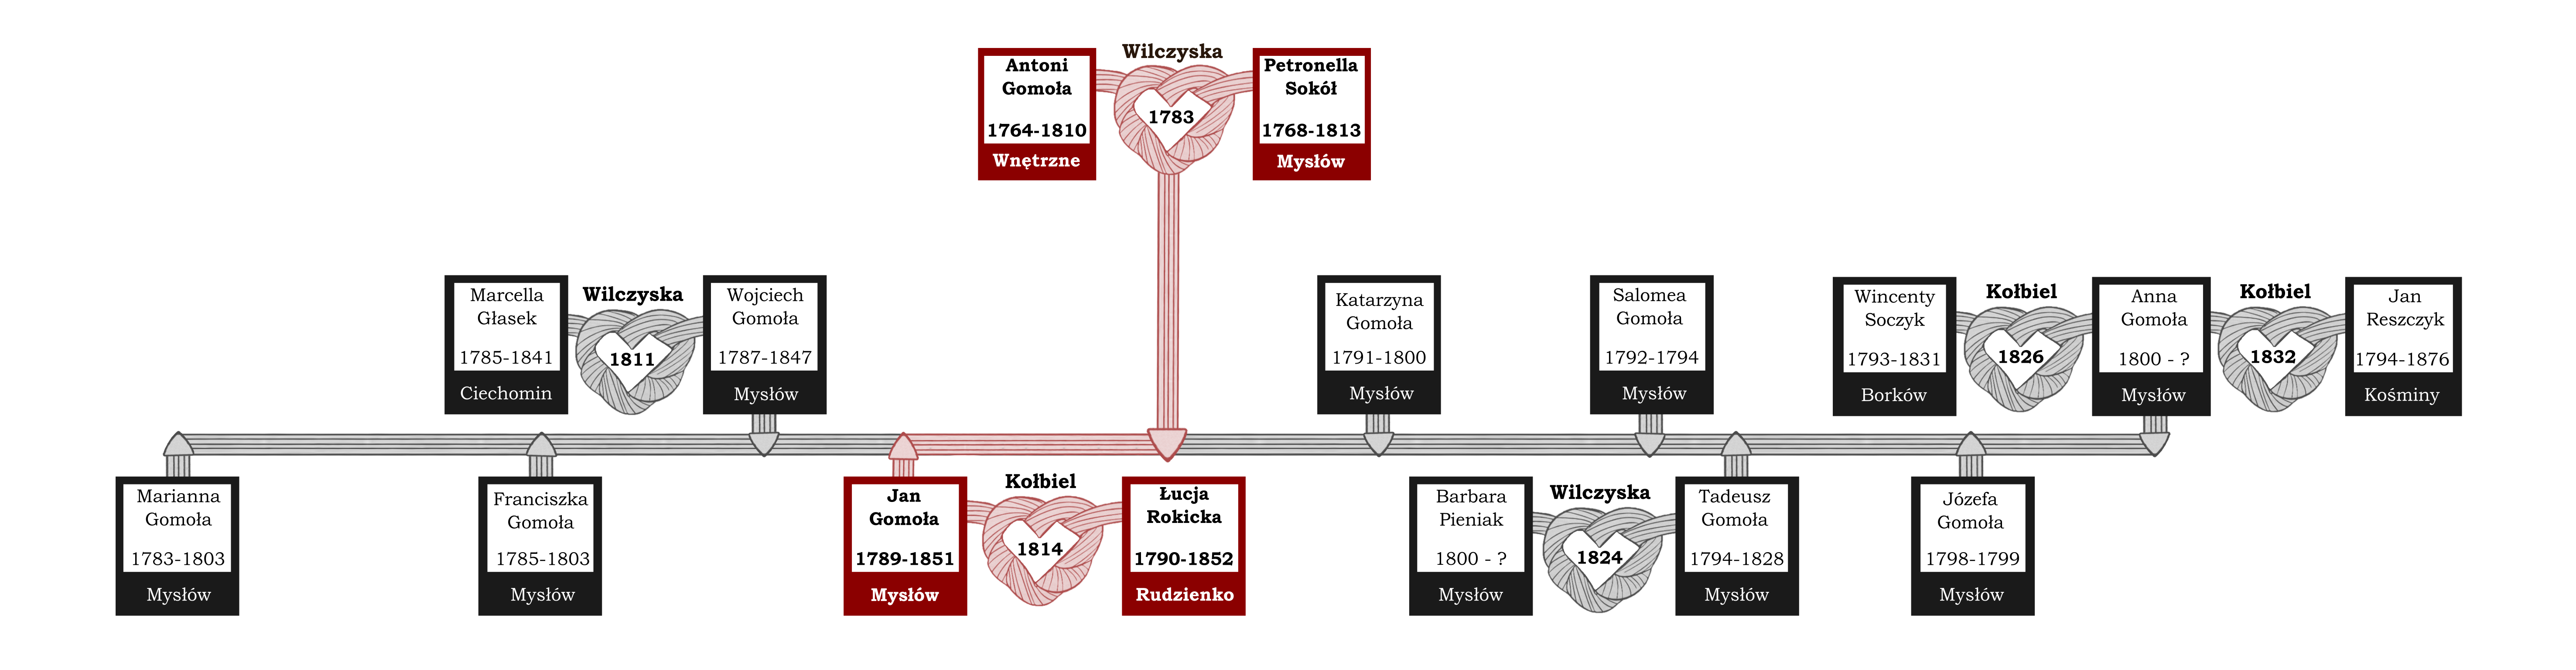
\includegraphics[width=1.0\linewidth]{
        Drzewo - Pokolenie I-II.png}
    \captionsetup{format=hang}
    \caption{Drzewo genealogiczne rodziny Gomulskich - Pokolenia I-II.}
\end{sidewaysfigure}